\documentclass[12pt]{article}
\usepackage{graphicx} % Required for inserting images
\usepackage{tabularx}
\usepackage{booktabs}
\usepackage{parskip}
\usepackage[a4paper, margin=1.5in]{geometry}

\newcommand{\desctotoc}[1]{%
  \addtocontents{toc}{\medskip\noindent\detokenize{#1}\leavevmode\par\medskip}
}


%% Common Parts

\newcommand{\progname}{Scanalyze AI} % PUT YOUR PROGRAM NAME HERE
\newcommand{\authname}{Team 16, Ace
\\ Hamza Issa
\\ Ahmad Hamadi
\\ Jared Paul
\\ Gurnoor Bal} % AUTHOR NAMES                  

\usepackage{hyperref}
    \hypersetup{colorlinks=true, linkcolor=blue, citecolor=blue, filecolor=blue,
                urlcolor=blue, unicode=false}
    \urlstyle{same}
                                


\begin{document}

\title{User Guide for Scanalyze AI}
\author{\authname}
\date{\today}

\maketitle
\pagenumbering{arabic}

~\newpage

\tableofcontents

~\newpage

\section*{Revision History}

\begin{tabularx}{\textwidth}{p{3cm}p{2cm}X}
\toprule {\textbf{Date}} & {Author} & {Section}\\
\midrule
4 April & Hamza & All sections, finished creating User Guide\\
4 April & Harrison & Edited all sections, added Login and FAQs\\
\bottomrule
\end{tabularx}

~\\

~\newpage

\section{Introduction}
\desctotoc{Overview of the Scanalyze Imaging Platform and its intended use by radiologists.}

Welcome to the user guide for the Scanalyze Imaging Platform, an advanced AI-powered tool designed specifically for radiologists. This platform allows medical professionals to upload chest X-ray (CXR) images and receive automated diagnostic support, including disease prediction, comprehensive report generation, and interactive visual analysis tools.

The goal of this platform is to assist radiologists in their workflow by providing accurate, explainable outputs that complement professional clinical judgment. While this tool leverages advanced machine learning algorithms to generate insights, it is intended for use as a decision-support system, not a replacement for a formal radiologic diagnosis.

This guide covers the full range of platform functionality, from account creation and image upload to interpreting AI-generated reports, exploring image findings, and downloading clinical summaries.

\newpage

\section{Signup}
\desctotoc{Instructions for creating a new user account, including required fields and system validation.}

The first step to using the platform is creating your account.

\subsection{How to Sign Up}

On the signup page, you will see a registration form like the one shown below:

\begin{center}
    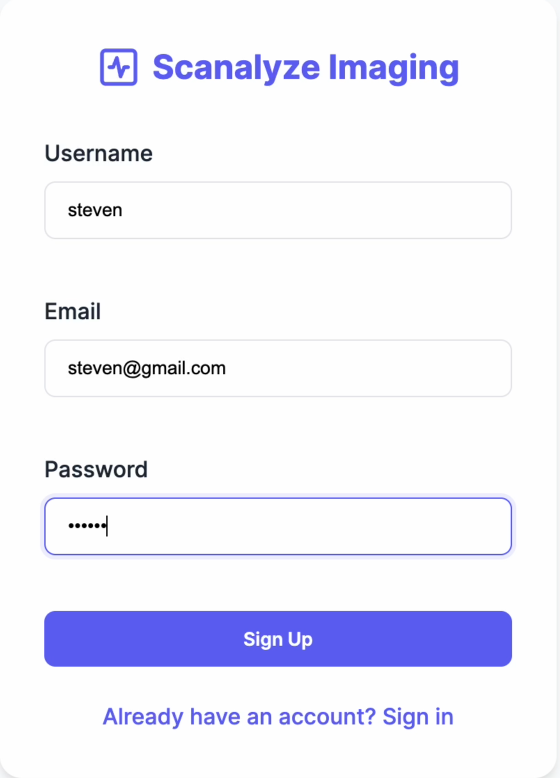
\includegraphics[width=0.35\textwidth]{scan1.png}
\end{center}

To complete the signup process:

\begin{enumerate}
    \item Enter your Username -- this will identify you on the platform.
    \item Enter a valid Email address -- make sure the email is correctly formatted (e.g., \texttt{name@example.com}).
    \item Enter a secure Password -- choose a strong password that you will remember.
    \item Click the Sign Up button.
\end{enumerate}

\subsection{What Happens Next}

\begin{itemize}
    \item If your input meets the platform's requirements (unique email, valid format, and acceptable password), you will be automatically redirected to the login screen.
    \item If any of the fields contain invalid or duplicate information, the system will notify you to make corrections before you can proceed.
\end{itemize}

After successful registration, you can log in and begin using the platform to analyze chest X-rays.

\newpage


\section{Login}
\desctotoc{Steps to log in to the platform using your registered credentials.}

\subsection{How to Log In}
\begin{enumerate}
    \item Navigate to the login page of the platform.
    \item Enter your registered Email Address in the email field.
    \item Enter your Password in the password field.
    \item Click the Login button to access your account.
\end{enumerate}

\begin{center}
    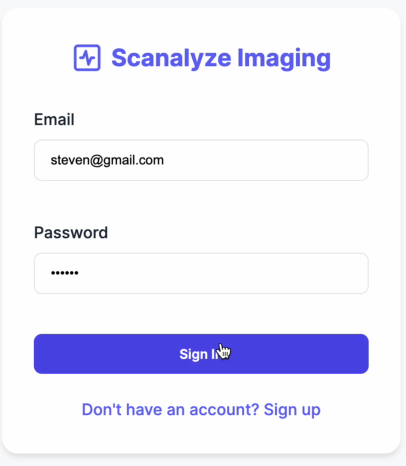
\includegraphics[width=0.7\textwidth]{scan8.png}
\end{center}

\subsection{What Happens Next}
\begin{itemize}
    \item If the credentials are correct, you will be redirected to the Model Selection page, where you can choose the diagnostic tool you want to use.
    \item If the credentials are incorrect, an error message will appear stating, "Invalid email or password. Please try again."
\end{itemize}

\subsection{Important Notes}
\begin{itemize}
    \item Ensure that you use the same email address and password you registered with.
    \item For security reasons, the platform enforces a maximum of 5 failed login attempts before temporarily locking the account. If this happens, wait 15 minutes before trying again or contact support for assistance.
\end{itemize}

\section{Select Model}
\desctotoc{Guide to choosing the appropriate AI model (Chest X-Ray Analysis, Brain MRI Segmentation, Bone Fracture Detection) and proceeding to analysis.}

After logging in, you will be directed to the platform's Model Selection page. This page allows you to choose from several AI-powered diagnostic tools tailored for different types of medical imaging.

\subsection{Available Models}

The available models include:

\begin{itemize}
    \item Chest X-Ray Analysis: Detects various chest conditions, including pneumonia, COVID-19, and other abnormalities.
    \item Brain MRI Segmentation: Identifies and segments brain tumors and lesions from MRI scans.
    \item Bone Fracture Detection: Detects fractures and abnormalities in X-ray images of bones.
\end{itemize}

\subsection{How to Proceed}

To analyze a chest X-ray image:

\begin{enumerate}
    \item Locate the Chest X-Ray Analysis card.
    \item Click on the "Chest X-Ray Analysis" option.
\end{enumerate}

This action will take you to the CXR upload and analysis interface, where you can begin working with patient chest X-rays.

\begin{center}
    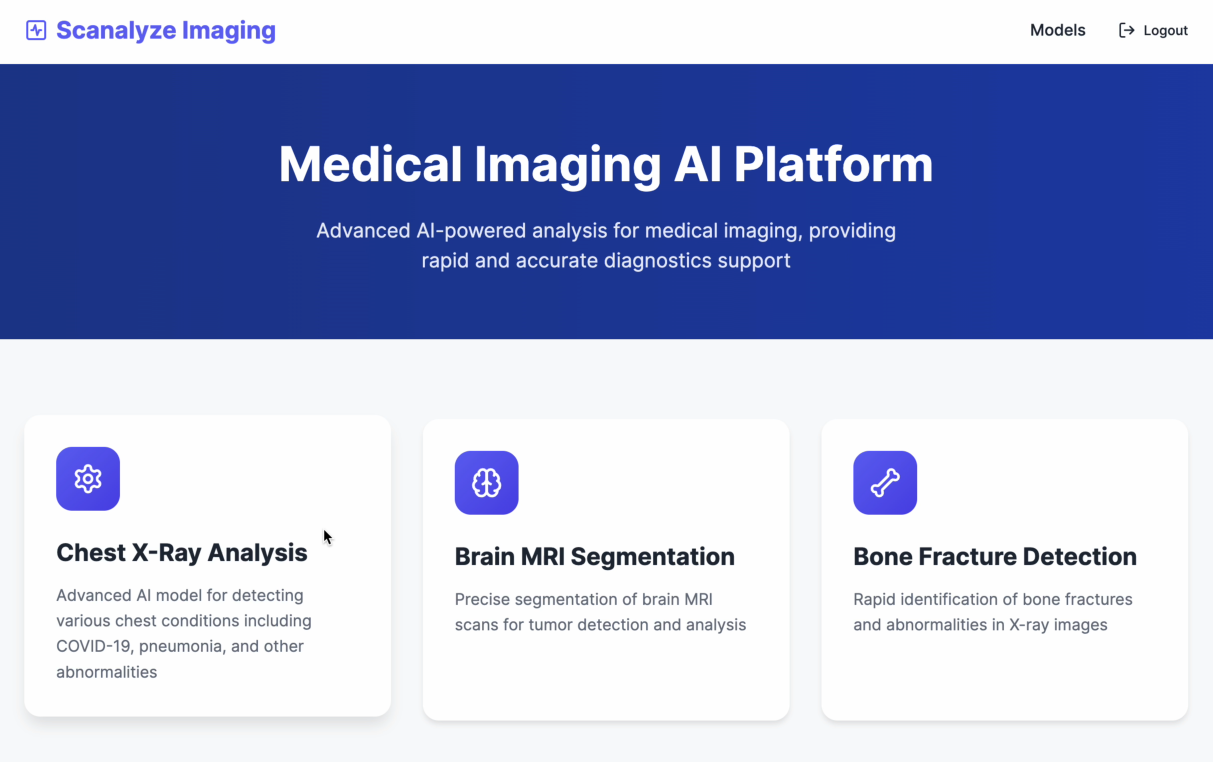
\includegraphics[width=\textwidth]{scan2.png}
\end{center}

\newpage

\section{Upload CXR Image}
\desctotoc{Instructions for uploading chest X-ray images using drag-and-drop or file selection.}

After selecting the Chest X-Ray Analysis model, you will be directed to the image upload page. This is where you submit the patient's chest X-ray (CXR) for automated analysis.

\subsection{How to Upload an Image}

The upload interface includes a clear image upload box, as shown below:

You can upload a medical image in either of the following ways:

\begin{itemize}
    \item Drag and drop your CXR image file into the upload area.
    \item Or, click the upload box to manually browse and select an image file from your device.
\end{itemize}

Once an image is uploaded, the platform will begin processing the file using its AI model.

\subsection{Important Notes}

\begin{itemize}
    \item Ensure the image is in a supported format (e.g., JPG, PNG, or DICOM).
    \item The AI system will generate predictions, a probability distribution of possible chest diseases, a detailed report of findings, and a visual explanation (e.g., heatmap) for interpretability.
    \item This tool is designed to assist with medical diagnostics and should not be used as a standalone diagnostic decision-maker.
\end{itemize}

A disclaimer is included at the bottom of the page stating that the tool is educational and should not replace professional clinical judgment.

\begin{center}
    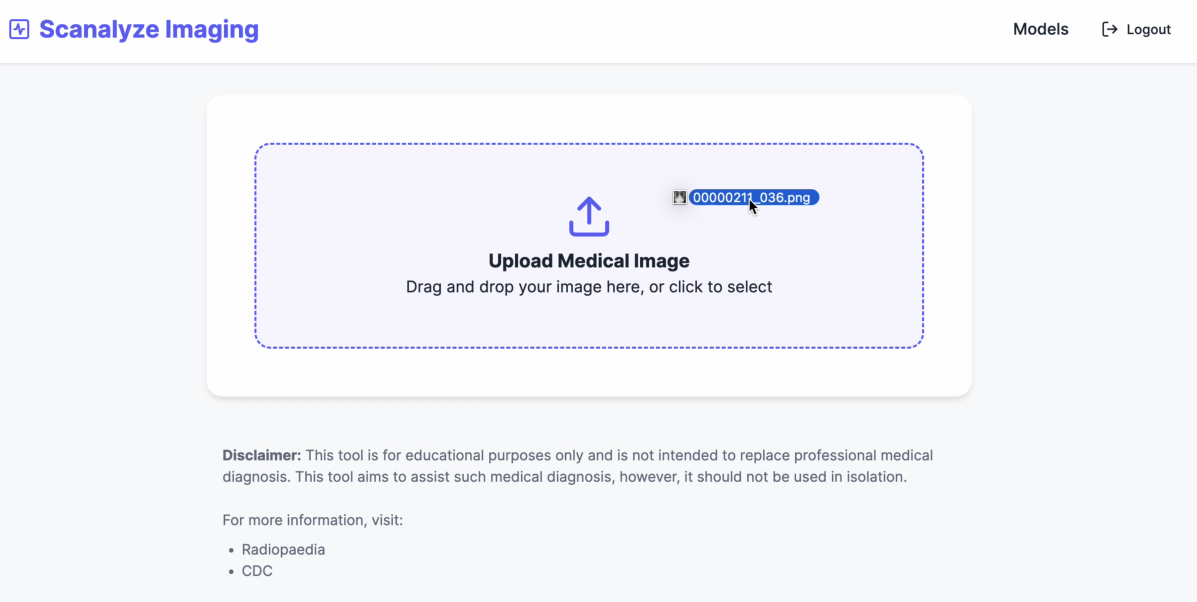
\includegraphics[width=\textwidth]{scan3.png}
\end{center}

\newpage

\section{Predicted Results and Report of Findings}
\desctotoc{Detailed breakdown of the AI-generated diagnostic report}


After a chest X-ray image is uploaded, the platform automatically performs an AI-based analysis and generates a comprehensive diagnostic report. This report is intended to assist radiologists in interpreting the model's findings with full transparency and interactivity.

\subsection{Report Overview}

Upon completion of the analysis, a completed report is displayed, including the following key components:

\begin{itemize}
    \item Timestamp indicating when the analysis was performed.
    \item A list of predicted findings based on the AI's highest confidence scores.
    \item Detailed medical descriptions of each predicted condition.
    \item A confidence slider to filter results.
    \item A probability distribution table of all considered diseases.
    \item A color-coded heatmap for quick visual interpretation of probabilities.
\end{itemize}

\subsection{Confidence Slider}

Located near the top of the report is the Confidence Threshold Slider, allowing users to adjust the minimum probability for a condition to be displayed.

\begin{itemize}
    \item Sliding right filters out lower-confidence predictions and shows only those with high certainty.
    \item This feature allows radiologists to tailor their level of diagnostic confidence based on their clinical context, focusing only on the most probable conditions if desired.
\end{itemize}

\subsection{Findings}

Immediately below the confidence slider, the model's most likely conditions are listed under "Findings." These represent the diagnoses with the highest probabilities. For example, in the displayed report, the model has identified Effusion and Edema as the top findings.

\subsubsection*{Description of Predicted Conditions}

Each predicted condition is accompanied by a detailed explanation, which includes:

\begin{itemize}
    \item Clinical definition: Explaining what the disease is and its implications (e.g., edema is fluid accumulation often seen in congestive heart failure).
    \item Radiologic description: Highlighting how the disease typically appears on a chest X-ray (e.g., bathing opacities, Kerley B lines, or blunting of the costophrenic angle).
\end{itemize}

These descriptions help radiologists compare the AI findings with their own image interpretation, strengthening the diagnostic decision-making process.

\subsection{Probability Distribution Table}

The system provides a detailed probability distribution of all analyzed disease classes. Each condition is shown with its associated percentage, representing the model's confidence.

\begin{itemize}
    \item This table is sorted to emphasize high-confidence predictions while also revealing lower-likelihood conditions for full transparency.
    \item It is particularly helpful when considering differential diagnoses and diagnosing conditions with low probability.
\end{itemize}

\subsection{Heatmap Visualization}

Beneath the probability table, a heatmap view provides a fast and intuitive way to interpret disease probabilities.

\begin{itemize}
    \item Conditions are presented as color-coded boxes, ranging from red (high probability) to green (low probability).
    \item This allows for quick visual assessment of the disease, with higher probability conditions (e.g., Effusion at 66.5\%) shown in red, while less likely ones (e.g., Emphysema at 7.85\%) appear in green.
    \item The heatmap components this numerical data, offering an auto-glance summary that enhances situational awareness.
\end{itemize}

\begin{center}
    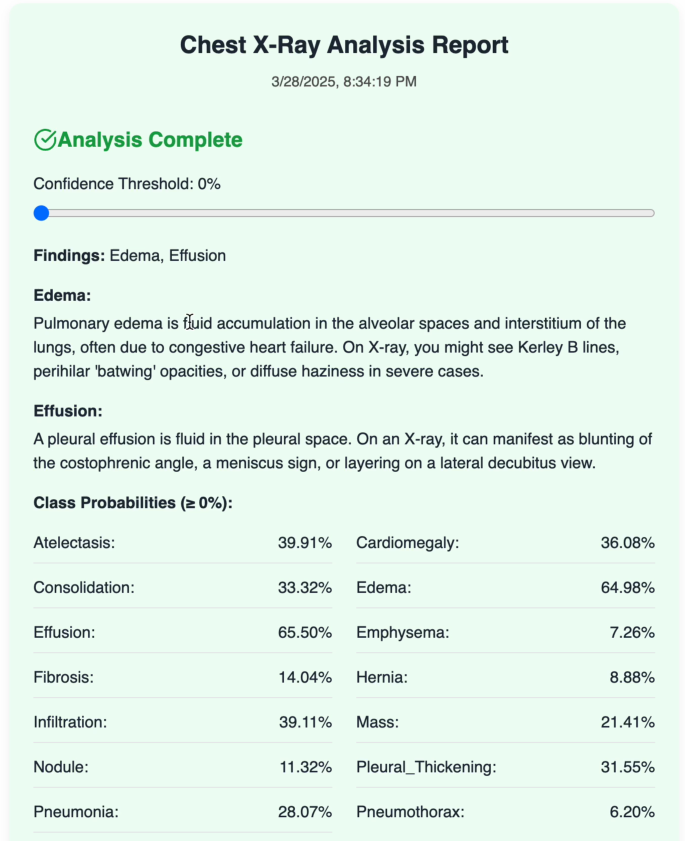
\includegraphics[width=0.7\textwidth]{scan4.png}
\end{center}

\begin{center}
    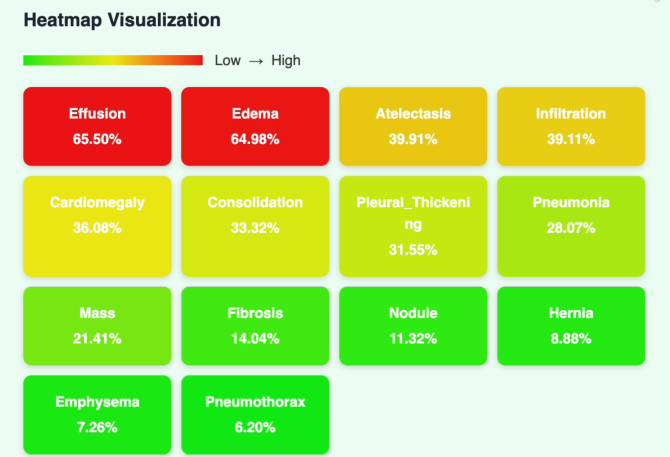
\includegraphics[width=0.7\textwidth]{scan5.png}
\end{center}

\newpage

\section{Exploring the CXR Image}
\desctotoc{Interactive features for zooming and dragging the image to explore AI-highlighted findings.}

Once the AI has completed its analysis and generated the report, the original chest X-ray (CXR) image is displayed on the screen. This image viewer is equipped with interactive tools to allow detailed inspection by radiologists.

\subsection{Interactive Tools for Image Exploration}

Radiologists can explore the CXR image using the following built-in tools:

\begin{itemize}
    \item Zoom Functionality: You can zoom in on specific areas of the X-ray for a closer inspection. This is especially helpful when reviewing image findings mentioned in the report, such as observing Kerley B lines, fluid levels, or lung opacities.
    \item Drag-to-Pan: After zooming in, you can click and drag the image to move across different regions of the scan. This allows you to focus on particular anatomical structures or abnormalities in detail, without losing your place.
    \item Responsive Exploration: The viewer responds smoothly to mouse scroll or trackpad pinch gestures for zooming, and click-drag gestures for panning, mimicking a diagnostic workstation experience.
\end{itemize}

\subsection{Practical Use}

These interactive tools are designed to support and enhance the interpretation of the report findings. For example:

\begin{itemize}
    \item If the report highlights effusion, the radiologist can zoom in on the lower lung fields or costophrenic angles to confirm fluid levels.
    \item If edema is noted, the upper and mid-lung zones can be inspected more closely for classic patterns such as vascular redistribution or perihilar haze.
\end{itemize}

The goal is to give radiologists the control to visually verify and explore AI-generated predictions within the image itself.

\begin{center}
    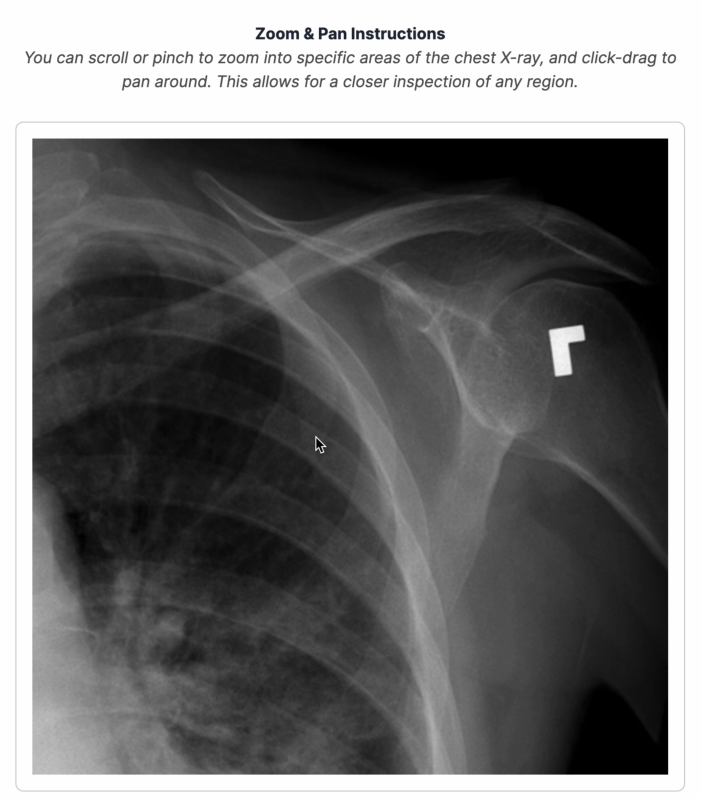
\includegraphics[width=0.9\textwidth]{scan6.png}
\end{center}

\newpage

\section{Download Report}
\desctotoc{How to generate and save a complete PDF report including findings, descriptions, probability scores, heatmap, and confidence settings.}

After reviewing the full analysis, radiologists have the option to save a complete copy of the findings using the Download Report button.

\subsection{Purpose of the Report}

The downloadable report serves as a comprehensive summary of the AI analysis and is suitable for:

\begin{itemize}
    \item Storing in patient records for documentation or follow-up.
    \item Sharing with colleagues for consultation or second opinion.
    \item Archiving for research or institutional case tracking.
\end{itemize}

\subsection{What the Report Includes}

When the Download Report button is clicked, a formatted PDF file is generated containing all key diagnostic information:

\begin{itemize}
    \item Timestamp of when the analysis was completed.
    \item Predicted findings selected by the AI model.
    \item Detailed medical descriptions of the predicted conditions, including radiographic cues.
    \item The full probability distribution table showing the AI's confidence scores for all possible conditions.
    \item The confidence threshold setting used at the time of analysis.
    \item The heatmap visualization summarizing likelihoods in a color-coded format.
\end{itemize}

This PDF mirrors the information seen on-screen, ensuring nothing is lost or omitted in the export.

\subsection{Using the Button}

\begin{enumerate}
    \item Once the analysis report is displayed, locate the Download Report button near the bottom of the interface.
    \item Click the button to begin the download.
    \item The report will be saved to your local system in PDF format, ready for use in clinical documentation or further review.
\end{enumerate}

This feature ensures radiologists can retain and share a consistent, clear, and complete copy of the AI findings at any time.

\begin{center}
    
\includegraphics[width=0.9\textwidth]{scan7.png}
\end{center}

\section{Frequently Asked Questions (FAQ)}
\desctotoc{Common questions regarding usage, data formats, diagnostic value, and technical features of the platform.}

\subsection{General Questions}
\subsubsection{What is the purpose of the Scanalyze Imaging Platform?}
The platform is designed to assist radiologists by providing AI-powered diagnostic support for chest X-rays, including disease predictions, probability distributions, and visual explanations.

\subsubsection{Is this platform a replacement for a radiologist's diagnosis?}
No, the platform is a decision-support tool meant to complement professional clinical judgment, not replace it. Radiologists should always verify AI-generated predictions with their own experience and knowledge.

\subsection{Usage Questions}
\subsubsection{What image formats are supported for upload?}
The platform supports JPG, JPEG, and PNG formats.

\subsubsection{How long does it take to analyze an image?}
The analysis typically takes less than 5 seconds, depending on the image size and server load.

\subsubsection{Can I use the platform on mobile devices?}
Yes, the platform is optimized for both desktop and mobile browsers.

\subsection{Technical Questions}
\subsubsection{What happens if the platform cannot process my image?}
If the image is unsupported or corrupted, an error message will appear. Ensure the image is in a supported format and try again.

\subsubsection{How secure is my data?}
The platform uses AES-256 encryption for data storage and transmission, ensuring your data is secure.

\subsubsection{Can I download the analysis results?}
Yes, you can download a comprehensive PDF report of the analysis using the "Download Report" button.

\subsection{AI and Diagnostic Questions}
\subsubsection{How accurate are the AI predictions?}
The AI model has been trained on a large dataset (NIH chest xray dataset) which has over 100,000+ images. It has 70\%+ AUC ROC score which means it can discriminate between an existence of a disease and the non-existence of one well. However, predictions should always be verified by a radiologist.

\subsubsection{What diseases can the AI detect?}
The AI can detect 13 different conditions: Atelectasis, Cardiomegaly, Consolidation, Edema,
Effusion, Emphysema, Fibrosis, Infiltration, Mass, Nodule, Pleural Thickening, Pneumonia, and Pneumothorax.

\subsubsection{What should I do if the AI gives low-confidence predictions?}
If the confidence scores are low, consult a radiologist for further evaluation.


\end{document}